% !TEX encoding = utf8
% !TEX root = ../main.tex

% This content has been generated automatically from https://www.docx2latex.com/docx2latex_free and https://github.com/MartinoMensio/doc2latex_process_chapters 
% Consider editing the source Google Doc instead of this one!


\chapter{Implementation}
\label{implementation}

This chapter focuses on the bot prototype that has been developed to put in practise the studies that have been done. This chapter reports the things that have reached the implementation stage. The implementation can be divided in two main areas:

\begin{itemize}
	\item Multichannel implementation: platform-dependent code completely decoupled from the core of the bot;

	\item Natural Language Understanding: the implementation of recurrent neural network for joint intent detection and slot filling in single and multi-turn environments.
\end{itemize}

As mentioned previously the personalization part remained as a draft only and is not active in the prototype.

While the first part is really bound to the bot scenario, where it is important to interface with the messaging platforms, the second one can also be used as a standalone framework to evaluate performances on different datasets.

The whole implementation of the system is available as a open source repository,\footnote{\url{https://github.com/D2KLab/botcycle}} that contains two modules: one dedicated to the specific bot for the bike sharing, while the other is relative to the Natural Language Understanding and neural networks.

\section{Interaction with chat platforms}
\label{implementationInteraction}

To interact with the chat platforms it was mentioned that a separate component has been designed to adapt to the different messaging platforms. This component, the Bot Server, on one side communicates with the Bot Core, that can be physically hosted on another machine, and on the other side interfaces with messaging platforms.

The overall architecture of all the distributed components can be viewed in Figure~\ref{fig:physicalComponents}. In this figure different types of components can be seen. On the left the user devices are shown, that can interface with different messaging platforms and websites. Those red components, the channels, are not manageable from the bot developer. Usually an account is built for the bot, but the communication with the user is completely handled by the reference platform. A special case is played by the website in blue, that provides an additional platform to chat with the bot without requiring any messenger accounts. Going a bit on the right, we can see the concentration role of the Bot Framework server that handles dishomogeneous data on the left and transforms them to a more standardized form on the right. This component is configurable by the bot developer, who through a web graphical interface can add and configure the channels on the left and at the same moment configure the external webservice on the right (the Bot Server). The Bot Server, under the full control of the developer, applies extra transformations of messages and plays also the role of a web server. The intelligent part, containing the Bot Core, is deployed on another machine without being reachable from the outside.

%%%%%%%%%%%%%%%%%%%% Figure/Image No: 32 starts here %%%%%%%%%%%%%%%%%%%%

\begin{figure}[!htbp]
    \centering
    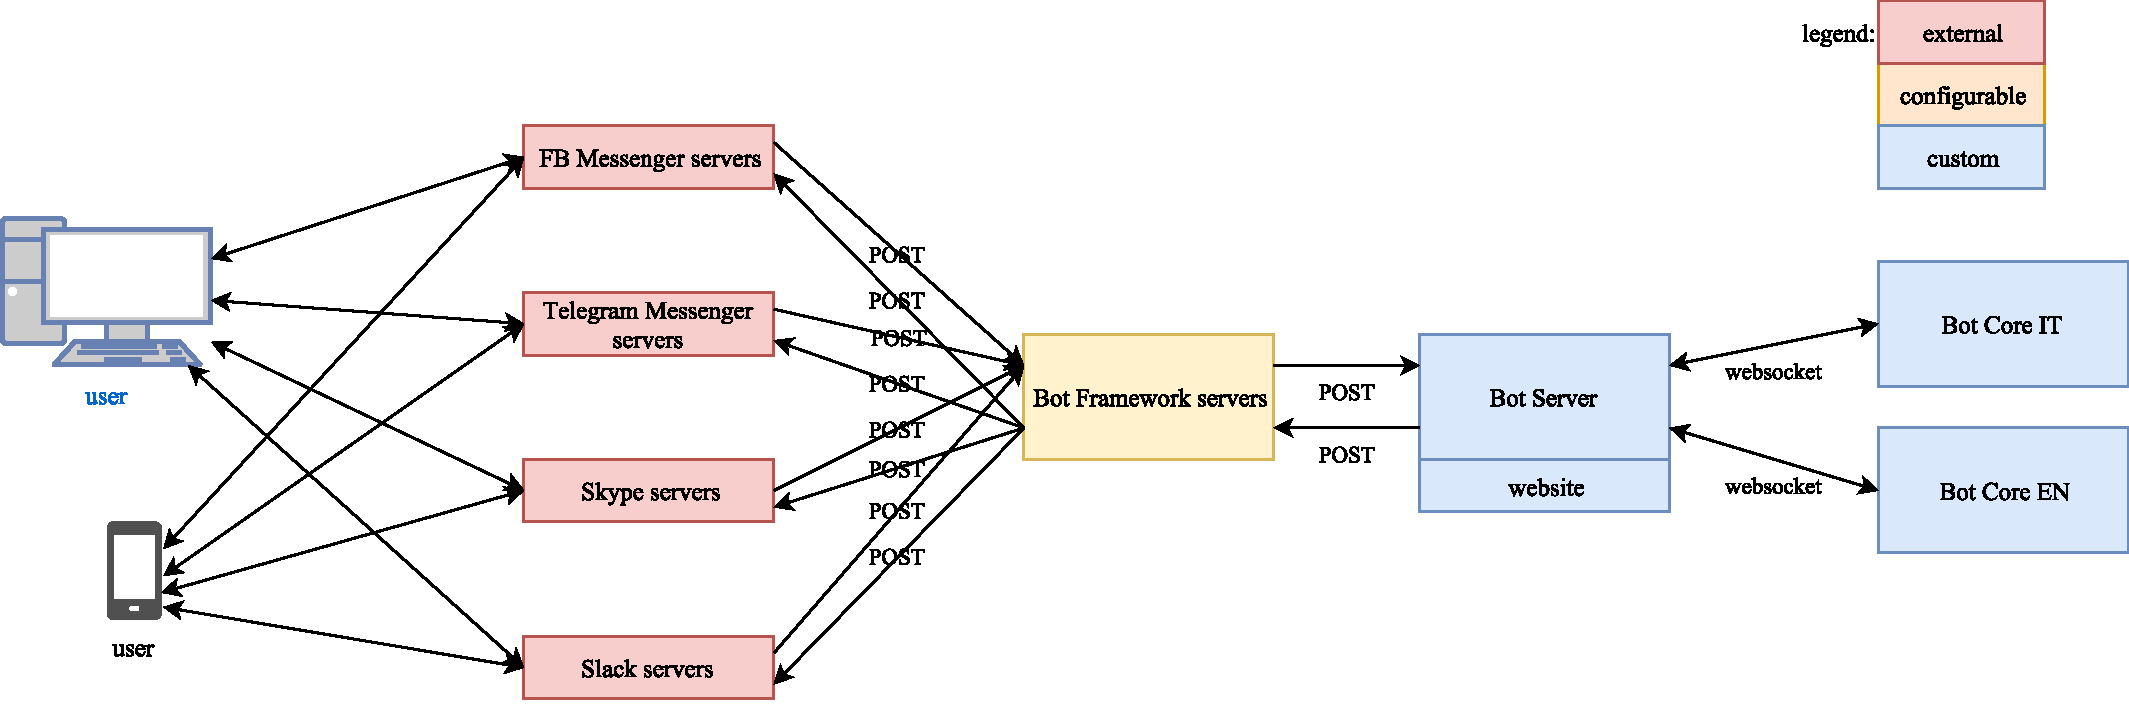
\includegraphics[max width=\linewidth,max height=8cm,keepaspectratio]{figures/physicalComponents}
    \caption{The physical components involved}\label{fig:physicalComponents}
\end{figure}

The communication between the two custom components (in blue in the figure) is done over a websocket to allow asynchronous messages to be sent in both directions, without using polling techniques that may consume resources and bandwidth. The Bot Server exposes two different endpoints for Bot Cores, one for the English version and one for the Italian one. Those endpoints thanks to HTTPS protocol offer a reliable channel that provides data encryption to protect data in motion and authentication through a symmetric key shared between the two parts. The data is transferred between those two components with the JSON standard over the websocket, with a format that does not depend on any specific messaging platform.

The Bot Server is not put directly in contact with the Messaging platforms because it would have required to implement all the webhook endpoints for them and also to translate from and to all the platform dialects. The most easy way to implement it has been found by interacting with a third-party component (Microsoft Bot Framework) that can be configured on a web portal to reach the different platforms. This removed a lot of implementation effort but brought to an architecture that is not very elegant and compact. The communication between the Bot Server and the Bot Framework is done in a way that is similar to the one required by messaging platforms: both components expose web endpoints (that must provide HTTPS connections with digital certificates that have as root a trusted CA) that are used for one-directional communications (the only response that is given is a status code that represent the outcome of the request) and each message is sent independently in its direction.

The supported platforms that have been configured for users to chat with the bot are the following:

\begin{itemize}
	\item Telegram: chosen because it is easy to create bots and is a $``$must$"$  for historical reasons. This channel is available both for English\footnote{\url{https://telegram.me/botcycle\_bot}} and Italian\footnote{\url{https://telegram.me/botcycle\_it\_bot}} languages. A particularity of this platform is that it allows using a special kind of buttons that enables the user to send his current location.

	\item Facebook Messenger: chosen because linked to Facebook it is one of the messaging platform with the biggest number of potential users. This channel too is available both in English\footnote{\url{https://m.me/BotCycleEn}} and Italian\footnote{\url{https://m.me/BotCycleIt}} languages. Similarly to what happens on Telegram, a special button can be built with the capability to pick a location on a map.

	\item Skype: exploiting the exclusive Bot Framework support for the platform, that is not usable otherwise, this channel is added both for English\footnote{\url{https://join.skype.com/bot/2cb007d1-5dd5-441a-8503-23268e2df32d}} and Italian.\footnote{\url{https://join.skype.com/bot/db2aa777-2e46-40fc-9e49-9bc9d1db201b}} However the majority of people do not even know that bots can live on skype.

	\item Slack: used for internal experimental testing on a dedicated workspace.

	\item Web site: a dedicated website\footnote{\url{https://botcycle-server.herokuapp.com/}} allows to test the bot without using messenger apps.
\end{itemize}

The main role of the Bot Server is to receive the messages on one side and provide them to the other one, by transforming their representation. The Bot Framework works well in the direction of receiving the messages from the user, but on the other directions does not provide all the features specific to the messaging platform. For instance, both on Facebook Messenger and on Telegram, buttons can be shown to the user in order to send the current position, while other platforms do not support it. To send these types of messages, it is necessary to send attachments in the native form of the platform ('\textit{quick\_replies}' with \textit{'content\_type': 'location'} for Facebook, \textit{'reply\_markup'} with \textit{'request\_location': true} for Telegram). Furthermore, this component also provides a web page where users can test the bot without using messaging platforms, as has been described previously. Also the Bot Server source code is made available openly,\footnote{\url{https://github.com/MartinoMensio/botcycle-server}} and makes internally usage of the Botkit library\footnote{\url{https://botkit.ai/}} to interface correctly with the Bot Framework.

Having two different custom components has many advantages: both conceptual and practical. The main conceptual advantage is that the coupling with messaging platforms is reduced: the bot core does not know anything related to them, and interacts with a representation of data that is human-readable and has no dependencies. The practical ones are many, generated from different needs, first of all performance. The Bot Server does not require high computation resources because is simply a proxy that manipulates the representation of information. The Bot Core instead, running Neural Networks to classify the sentences, needs disk space and RAM (the language models are quite huge), together with a computing power that should be sufficient to produce outputs in short times. The Bot Server instead requires to host a web server with a fixed hostname and with good certificates provided by a CA trusted from the Bot Framework. This hostname needs to be configured as a webhook endpoint to whom send POST requests with the incoming messages.

Having those needs and opting for a cheap feasible option (without buying a powerful VPS with all those features), the choice has been to split those components. The Bot Server is hosted on heroku\footnote{\url{https://www.heroku.com/}} with a free plan that has limitations in computing power and space, but fits the requirements for this component. Especially, the platform supports natively HTTPS that are covered by a wildcard certificate (every application receives a URL that matching with \textit{$\ast$ .herokuapp.com} is covered). Websites and Web Server applications can easily be created (using one of a large set of supported languages and frameworks) and pushed to the platform and the deployment will occur with no pains in configuration. Having the websocket endpoints exposed on the Bot Server, the Bot Core does not require to act as a server: no hostname is required, no certificate, no port forwarding on NATs, no ports open on the machine that runs it. This enforces a lot the security of the system. Furthermore also the websockets are HTTPS as offered by the Bot Server, so no plaintext interactions can be intercepted.

To make clear how all the components work together, let us follow what happens from when a user sends a message until he receives back a response. First of all, the user connected to a messaging platform (Facebook Messenger) sends some text, that arrives to the Facebook Servers. From there, since the destination account is a page that has been configured to receive messages at a certain webhook location, the message is sent to the Bot Framework. From the Bot Framework, the message is forwarded to the Bot Server that is finally one of the two custom components that has been developed. The Bot Server, checking that a Bot Core is connected over websocket for the specific language, delivers the message. The Bot Core processes the message (NLU, Information Retrieval, Response Generation) and replies on the websocket. The Bot Server transforms the response for the dialect of the destination platform and forwards the message to the Bot Framework that delivers it to the Facebook Servers. Finally the user receives the message.

The flow is quite intricate but has all the advantages listed above.

\section{Natural Language Understanding}
\label{implementationNLU}

This section focuses on the implementation that has been done relatively to the Natural Language Understanding described on the previous chapter \ref{approachNLU}. Firstly, a description is done of the external NLU provider that has been used to initially handle the understanding process and successively has been kept as a single-turn dataset collector and manager (\ref{implementationWit}). Then the discourse will cover some details about the frameworks used for implementing the neural networks in \ref{implementationNN}, and also about some specific issues risen in the development in \ref{implementationNNDetails}. A dedicated subsection is then given to word embeddings in \ref{implementationWV} and the last part explains how the datasets have been collected and preprocessed to uniformly be fed to the neural network in \ref{implementationDatasets}.

\subsection{Wit.ai exploitation}
\label{implementationWit}

In the early stages of the bot, the Natural Language Understanding has been delegated to an external provider: wit.ai.\footnote{\url{https://wit.ai/}} It was chosen for its simplicity to use and for being a standalone product that just provides NLU usable through a web API.

While giving the advantage to have an almost ready to use NLU (the configuration of intents and entities requires few steps and few examples), it also helps building a dataset. All the sentences that are sent for analysis are stored in a inbox, that can be analyzed and the responses can be interactively fixed and validated (inserted in the dataset). The dataset can also be downloaded, and because it is stored in comprehensible JSON format can be used as annotated dataset to later train another NLU system. A limitation of this service is that it handles only single-turn interactions, so the datasets that have been collected for both Italian and English languages can be only used for this type of interaction.

This stage of development has been done in order to understand the main needs of the users, and progressively new intents and examples have been added. On the other side, this experimentation also helped understanding what the NLU tasks are, giving an orientation in the very big landscape of Natural Language Processing. This helped directioning the study of literature towards approaches that could do a similar sentence classification and parameters extraction. During this stage, it has been noticed that for the intent classification task a promising approach is to use Recurrent Neural Networks, so the studies (both theoretical and practical) went deeper in exploring this field.

\subsection{Neural Networks frameworks}
\label{implementationNN}

As of today many open source libraries and frameworks are available for NLP tasks, using different programming languages and different approaches. The most important ones are:

\begin{itemize}
	\item Stanford Core NLP:\footnote{\url{https://nlp.stanford.edu/software/}} a java library that provides Tokenizer, NER, POS, Dependency Parsing, Coreference Resolution for languages: English, Arabic, Chinese, French, German, and Spanish;

	\item NLTK:\footnote{\url{https://www.nltk.org/}} a python library that focuses on Tokenizers, n-grams, POS, NER;

	\item Syntaxnet:\footnote{\url{https://github.com/tensorflow/models/tree/master/research/syntaxnet}} a neural-network NLP framework for TensorFlow. Helps building POS and Parsers. It contains pre-built models for POS and parsing. It is the most accurate parser for english, able to parse correctly garden-paths;

	\item SpaCy:\footnote{\url{https://spacy.io/}} an open source NLP framework that provides Tokenizer, NER, POS, Dependencies, Word Vectors, Parsing for different languages with the goal of being ready to use with pre-built models, and also fast.
\end{itemize}

But from what has been explored, those libraries focus on a selected subset of NLP tasks, and we wanted to implement Neural Networks to have full control of the process.

Experimenting with Neural Networks has become easier and easier in the last years thanks to open source libraries that provide high-level APIs and, being used more and more, the support is really easy to obtain on online communities (such as StackOverflow\footnote{\url{https://stackoverflow.com/}}) or on the official documentation or directly on the official code repositories (by means of interlined comments or $``$\textit{self-documenting code}$"$~\cite{raskin2005comments}). The programming languages that are supported for Neural Networks are many, but the most used nowadays is Python. In Python the most used frameworks are Keras\footnote{\url{https://keras.io/}} and TensorFlow.\footnote{\url{https://www.tensorflow.org/}}

For choosing between Keras and Tensorflow, experiments have been done with both. It is important to say that the two frameworks are not uncorrelated, because Keras as default backend uses TensorFlow and TensorFlow recognizes Keras as its high-level interface.\footnote{\url{http://www.fast.ai/2017/01/03/keras/}} So the problem is simply to choose the abstraction level desired.

Initially, when trying to emulate a RNN approach for Intent Classification (see section \ref{soaIntent}, Keras has been used to implement it. Without considering the data preprocessing part that is needed to get the desired shape and values for the inputs and outputs (as inputs word vectors corresponding to the words in the sentence and as outputs the corresponding intent type), the building of the computation graph (a bidirectional LSTM layer followed by a densely connected layer) and its training just required few lines of code.

But when trying to implement less regular models, such as the encoder-decoder of~\cite{liu2016attention}, the criticality of using only high level API came out, especially considering complex parts like output dependencies.

For this reason a comparison has been done in order to choose what implementation path to follow. Table~\ref{tab:kerasVsTf} summarizes the main differences found between Keras and TensorFlow.

%%%%%%%%%%%%%%%%%%%% Table No: 4 starts here %%%%%%%%%%%%%%%%%%%%

% !TEX encoding = utf8
% !TEX root = ../main.tex

\begin{table}
  \begin{tabularx}{\textwidth}{XXX}
    \toprule
    \textbf{feature} & \textbf{Keras} & \textbf{Tensorflow} \\
    \midrule
    Abstraction level & High & Can go down to reach single operations, but also high level API is provided by lots of classes \\
    \midrule
    Learning difficulty & Quite easy & More difficult, lots of details to consider \\
    \midrule
    Support for complex operations & Focuses more on simple regular layers and cells & Lot of already defined classes, and also helpers function that can help building complex operations \\
    \midrule
    Best for & Rapid prototyping & Advanced operations \\
    \midrule
    Documentation & Documentation good for what is implemented & Documentation gap between trivial and advanced \\
    \bottomrule
  \end{tabularx}
  \caption{A comparison between Keras and TensorFlow}\label{tab:kerasVsTf}
\end{table}

Let us see in more details what is the support provided by both libraries for building recurrent neural networks in the following paragraphs.

\subsubsection{Keras Recurrent API}
Similarly to what happens with feedforward neural network, also when working on recurrent ones handling Keras layers is like playing with LEGO:\footnote{\url{https://www.lego.com/}} blocks can be easily stacked one on the top of the other (also forks and joins are quite easy to perform). Keras Recurrent API is described extensively on its documentation,\footnote{\url{https://keras.io/layers/recurrent/}} while here only a quick overview is performed.

To define a recurrent layer in Keras the class \textit{keras.layer.RNN} takes as argument a RNN cell. Some parameters can be used to define how the layer will behave. A RNN cell is a class that has a call method that takes as input the actual input and the current state and produces the output and the next state. Different implemented cells exist.

\begin{itemize}
	\item \textit{SimpleRNNCell}: a cell that simply concatenates the input with the previous state and passes it through a feedforward layer;

	\item \textit{GRUCell}: Gated Recurrent Unit~\cite{cho2014learning};

	\item \textit{LSTMCell}: Long-Short Term Memory layer~\cite{hochreiter1997long}.
\end{itemize}

Layers can be easily stacked and the creation of deep recurrent network is very easy. Networks that are a simple stack of different layers (Recurrent, Dropout regularizations, Dense feedforward) will not find any problem in implementation. But when the networks are not so linear in the flow or when some advanced layers are required, there might not be an already implemented solution. For example there is no native implementation for \textit{seq2seq} models and layers, no \textit{Attention} mechanism and it is not possible to have a ready to use help for doing output dependency modeling (feeding back the outputs in a decoding layer). They can be implemented with the existing API, but they are not part of the library itself (some implementations can be found online,\footnote{\url{https://github.com/farizrahman4u/recurrentshop}} but the number of people working on it is order of magnitude smaller than the one involved in the TensorFlow community).

\subsubsection{Tensorflow Recurrent API}
Also tensorflow has classes for defining RNN layers and RNN cells. But there is more:

\begin{itemize}
	\item More cells: instead of a single implementation of LSTM and GRU, a wide variety of cells can be chosen

	\item More wrappers: wrappers can be used to encapsulate cells. DropoutWrapper, AttentionWrapper and a lot more can be added to the cells

	\item Seq2Seq native support: classes for defining encoders and decoders, with some helpers for modeling output dependencies can make a lot easier to build complex models that are not a linear chain of layers but contain links that move backwards in the stacked layers (as in output dependencies, where the output label is fed back to the decoder RNN). For example to build a decoder that considers output dependencies, in tensorflow three components are needed: a RNN cell (e.g. LSTMCell), a CustomHelper (that is responsible to provide values to the cell and take the outputs by simply declaring three custom functions) and a BasicDecoder that combines the cell with the helper and builds a layer. By dividing the roles of the cell and of the helper, a complex decoder can be built without a big effort.
\end{itemize}

More details about the available classes can be found in the official documentation of the seq2seq package.\footnote{\url{https://www.tensorflow.org/api\_docs/python/tf/contrib/seq2seq}}

\subsubsection{Decision}
The objectives of the decision between the frameworks are:

\begin{itemize}
	\item Ability to build the proposed network without too much headache. Especially for the decoding stage, some advanced wiring is needed and would like not to start from scratch (being really error-prone) but have some native support from the library;

	\item Code readability and maintainability: possibly using quite high level operations, no reinventing the wheel (in a buggy version)

	\item Quite good performances
\end{itemize}

Considering these objectives, the choice has been to use the native TensorFlow APIs for building the solution, using the seq2seq package for faster implementation. The additional work required to build even simple networks is compensated by the great flexibility of the library.

\subsection{Graph details}
\label{implementationNNDetails}

Implementing a neural network with tensorflow needs understanding some basic concepts.

First of all, the difference between defining a computational graph and actually doing operations. This is the concept of \textit{tensors}: they are a generalization of (multidimensional) vectors that will be used to contain values. Using and connecting them in computational graphs means defining how the values contained will be processed. The big difference with normal variables is the time of execution of the computations defined.

If in a programming language we have two variables  \( a=3,b=1 \)  and we sum them, when the instruction of sum is executed  \( c=a+b \)  the resulting variable will contain the result  \( c=4 \) . Instead defining a sum between tensors  \( a=tf.Variable \left( 3 \right) ,b=tf.Variable \left( 1 \right)  \) , when the instruction of  \( c=a+b \)  is executed the resulting tensor will not contain  \( 4 \) . It will be stored that c can be computed by summing what is contained in  \( a \)  and  \( b \) . In this way the operations can be defined once and the same computational graph can be run different times. To actually run the graph it is necessary to build a session, that is the execution environment. But in order to have different inputs to the same graph, there is the need to define the starting tensors not as Variables but as placeholders. Later when running the session, the placeholder values can be fed to the graph and the results can be evaluated. The library is powerful in how allows to define variables that can be initialized and automatically optimized by internally using the packpropagation of gradients. The only things that the programmer needs to do is to define the graph with all the tunable variables and declare a loss function to be optimized. No manual calculation of gradients, it is handled by TensorFlow.

The most difficult things to do while using this library are: \textit{(1)} know which operation to use, because there are so many classes available that only after a deep dive into documentation a solution is found; \textit{(2)} manipulate in the correct way multi-dimensional tensors, without making confusion. Both difficulties decrease by the increasing time used to experiment with it, but it is important to understand soon how to work with the $``$\textit{axes}$"$  parameter, crucial to perform reduction operation over the correct dimensions in nearly all the operations.

As has been discussed in the approach part, the chosen graph to be used in single-turn interactions is the encoder-decoder joint approach of~\cite{liu2016attention}. The paper comes with a TensorFlow implementation that is not complete:\footnote{\url{https://github.com/HadoopIt/rnn-nlu}} output label dependencies are not considered. Another negative property of the implementation is that it does not use a recent API, that would provide higher level functionalities and helper functions. Another implementation has been found that uses a more recent API and is really a lot more understandable that the original one.\footnote{\url{https://github.com/applenob/RNN-for-Joint-NLU}} It makes use of the \textit{seq2seq} native package,\footnote{\url{https://www.tensorflow.org/api\_guides/python/contrib.seq2seq}} that can be used for all the quite complicated networks that process sequences, like NMT or generative processing by employing classes that are relatively simple to use with respect to what they do.

So this last implementation has been used as starting point. Starting from this last implementation, that highly depend on the ATIS dataset~\cite{hemphill1990atis} in the preprocessing part, a slightly different implementation has been developed. The differences are described in the following paragraphs.

\subsubsection{The differences}
The main changes are not on the network structure, that is the one of the original paper, but in some details about the inputs and outputs.

First of all, the inputs of the computational graph, previously feeded as word indexes, have been changed to string tensors (that exist as native type in TensorFlow although its math-preponderance). In this way the dictionaries are part of the graph. Translation from word to indexes and the inverse operation is possible thanks to the package \textit{tf.contrib.lookup} that can be used to implement lookup tables for both the directions (words to indexes and indexes to words).

Then, having the lookup operations inside the computational graph and having the string tensors as inputs, it has been possible to define different ways to obtain the embedding values with the same interface. Both proceeding implementations contained the embedding matrix as a trainable Variable with size  \(  \left[ vocabulary \_ size  \times  embedding \_ size \right]  \) , and this embedding technique has been moved in a specific class. The other way to obtain the embedding values, that corresponds to pretrained fixed values, is to use an external library (SpaCy, see the details and implications below in word embeddings section \ref{implementationWV}) to get those values. The library requires words as parameters to get their representation, and it would not have possible to pass the word ids as in the previous implementation.

Having another class that wraps the external library call to get the embedding vectors, it is possible to test the two different approaches (trainable embeddings versus fixed pretrained embeddings) and some measures have been done showing a boost given by the second approach empowered by big corpora.

To make more understandable also the management of output dictionaries (intent types and IOB annotation types), the same strategy has been used. This time only trainable embeddings not precomputed have been used, because the words do not belong to the English or Italian dictionary (for example the word \textit{search\_bike} or \textit{B-location}).

The last kind of modifications that have been done are relative to saving the models trained and being able to resume them for inference time. This is possible thanks to the naming of tensors, that allows to save the computational graph and the values of the variables to the disk and resume it without re-defining all the variables that were present previously. To interact with the graph, it is possible to retrieve the input and output tensors by name and all the intermediate steps will be internally managed by TensorFlow. As will be described in \ref{implementationSpacyPyFunc}, the only parts that cannot be serialized are the external python functions, but a solution exists also for this problem.

\subsubsection{Multi-turn}
Relatively to the multi-turn implementation described in subsection \ref{approachMultiTurn}, the modifications for considering the previous agent turn are only on the preprocessing step, while for doing the top level intent RNN an addition has been done on the top of the intent logits. As can be seen in Figure~\ref{fig:approachMultiTurnDifferences}, instead of passing them to a softmax layer that estimates their value, the current turn intent logits are passed to a LSTM cell that receives as previous state the previous intent value. This specific point has been critical because the original idea was to propagate the previous state directly, as a vector of floating values, that would have allowed the backpropagation to go through the previous turns and optimize also tunable parameters of the past. But maintaining the state of this cell would have been difficult in the training phase specially. The training samples would have needed to be fed in the correct order (using the cell in stateful mode), or the whole discussion would have needed to be fed for each new user sentence. Both of these solution are not good for performance, so the decision has been to use directly the previous value of the intent instead of the state of the cell. This is something that is also done in sequence to sequence approaches, where previously generated words are fed as inputs to the decoding stages. In this case, the previous value of the intent is translated from string to an index (using the lookup table) and then transformed into a one hot encoding (a vector of zeros with a  \( 1 \) at the correct index).

%%%%%%%%%%%%%%%%%%%% Figure/Image No: 33 starts here %%%%%%%%%%%%%%%%%%%%

\begin{figure}[!htbp]
    \centering
    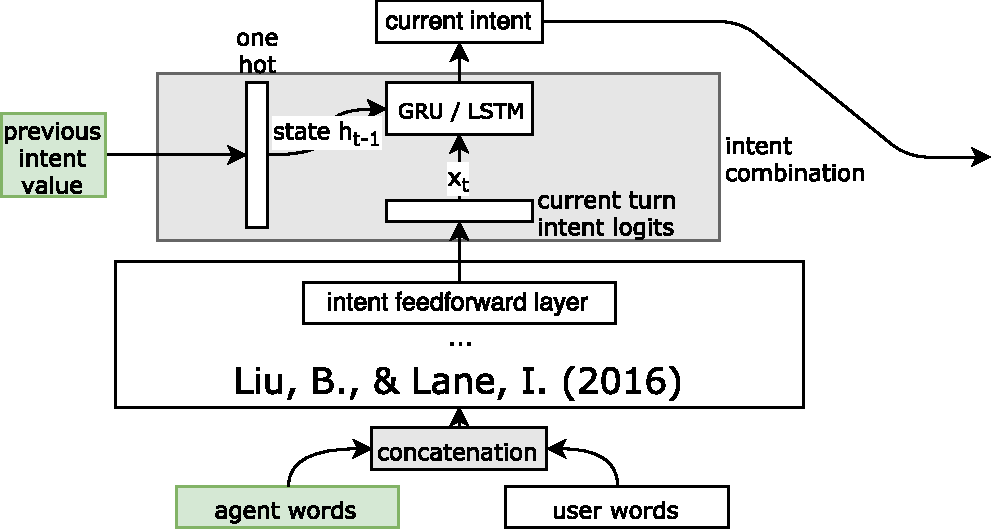
\includegraphics[max width=\linewidth,max height=8cm,keepaspectratio]{figures/approachMultiTurnDifferences}
    \caption{The differences of the multi-turn with respect to~\cite{liu2016attention}}\label{fig:approachMultiTurnDifferences}
\end{figure}

\subsection{Word embeddings}
\label{implementationWV}

To work with word embeddings different strategies and libraries can be applied. The most TensorFlow-purist one is to declare the embedding matrix (one vector for each word) directly as a TensorFlow variable. This is the simplest solution from word embeddings that are randomly initialized and are tunable. However it may have implementation and memory issues when the values come precomputed on bigger corpora (all the embedding matrix is loaded simultaneously in memory, and it is very important to keep only one copy of it in memory\footnote{\url{https://stackoverflow.com/questions/35687678/using-a-pre-trained-word-embedding-word2vec-or-glove-in-tensorflow}}). Furthermore, it is necessary to get the word embeddings from third party sources and manage the download of them carefully (the implementation presented in this work is based on docker containers\footnote{\url{https://www.docker.com/}} to provide high portability). And third party libraries can be necessary also to do common text processing or IOB label management.

For all these reasons, our implementation integrates a neural network library with a NLP library. For NLP, Spacy has been chosen for its good performances\footnote{\url{https://spacy.io/usage/facts-figures}} and models supporting word embeddings.\footnote{\url{https://spacy.io/models/}} It has been used also in an early stage of experimentation for identifying the entities with its native functionalities. The natively provided models come in different sizes, where the most spatial occupation is given by the word vectors. For example on the English language, four different models are available\footnote{\url{https://spacy.io/models/en}} where also the biggest one only occupies around 600MB.

For some other non-english languages only the smallest model is available, that does not contain precomputed word vectors. Instead, using character-based information, SpaCy provides contextual tensors\footnote{ https://spacy.io/usage/vectors-similarity$\#$ in-context  } that are estimated by applying a 4-level convolutional network sensitive to up to four words on either side of a word. The performances of these tensors are also analyzed in the validation chapter \ref{validationMeasures}, but generally they are not as good as word vectors precomputed on large corpora. However SpaCy allows quite easily to build new models that can integrate a native language model with externally computed word vectors.

\subsubsection{The tokenization of spaCy}
For splitting the sentences into words, with knowledge of the common problems explored in section \ref{soaVocabulary} when discussing about keeping or removing punctuation and special cases like apostrophes, the chosen approach is the one employed by the library SpaCy. This is done by applying rules specific to each language. Just as an example, punctuation is split off, like commas or periods at end of sentences, but "\textit{U.K.}" remains one token. English expressions like $``$\textit{don't}$"$  are tokenized into [$``$\textit{do}$"$ , $``$\textit{n't}$"$ ] and for this reason a lot of rules are applied. For other languages that do not have a full model, like the Italian one, the tokenization is more trivial because no one has yet worked on those rules. However it is always done better than a whitespace tokenization (splitting the words basing on spaces or other separator signs) combined with punctuation removal.

\subsubsection{Integrating SpaCy with TensorFlow}
\label{implementationSpacyPyFunc}

To integrate the Spacy NLP utilities inside a computation graph defined in TensorFlow, two different things have been done.

The first one is relative to the tokenization. To simplify the process of transform the sentences into vectors of words, it has been chosen to put this operation in the preprocessing step. A motivation for this solution is that the ATIS dataset~\cite{hemphill1990atis} has a predefined word tokenization based on whitespaces. To maintain the measurements comparable with other papers, in this specific case the tokenization is not modified while for other corpora, that only define sentences without saying how the words are separated, the SpaCy tokenization is applied. Having different tokenization models, to simplify the feeding of inputs the tokenization has been managed in the normalization procedure of datasets. The source datasets are preprocessed and saved to disk in a uniformed format (that can be seen in the \textit{preprocessed} folders\footnote{\url{https://github.com/D2KLab/botcycle/tree/master/nlu/data}}).

The second point of contact between the NLP library and the computational graph is established when the word embedding values are retrieved. Being inside the computational graph the only way to call a custom function, as a block that works with tensors, is to use the \textit{py\_func} helper. This method allows to put in the graph a python function, possibly idempotent to avoid side-effects that may generate unwanted behaviour since the training is usually done together with randomization of samples, that will receive and produce numpy arrays\footnote{\url{https://docs.scipy.org/doc/numpy-1.13.0/reference/generated/numpy.array.html}} translated back and forth to tensors for the graph.

The only problem of using this helper is that the graph will not be fully serialized to disk for future usage. The solution to this problem is to declare again the same function when the restoration of the graph and parameters are done, before declaring and using a running session.

\subsubsection{Italian word embeddings}
As has been said previously, for the Italian language, SpaCy has an incomplete model that does not contain precomputed word vectors but only contextual tensors (generated on the fly by a convolutional network) are available. For this reason, a side work has been done, taking the Wikipedia Italian corpus\footnote{\url{http://dumps.wikimedia.org/itwiki}} and computing GloVe vectors on it. Some preprocessing has been done to extract the text only of the dump with a mix of tools written by the SpaCy developers\footnote{\url{https://github.com/explosion/spacy-dev-resources}} and people from the University of Pisa.\footnote{\url{http://medialab.di.unipi.it/wiki/Wikipedia\_Extractor}} From the text, cleaned of all the markup and XML tags, a re-tokenization is applied to feed correctly the text to the GloVe algorithm.\footnote{\url{https://github.com/stanfordnlp/GloVe}} In this way both the dictionary and the tokenization used in the training of the word embeddings is the same that is used by the computational graph.

The output of this process is a SpaCy model that is made available openly\footnote{\url{https://github.com/MartinoMensio/it\_vectors\_wiki\_spacy}} and can be installed easily with \textit{pip}.\footnote{\url{https://pip.pypa.io/en/stable/}}

\subsection{Datasets collection}
\label{implementationDatasets}

This last subsection contains some details about how some datasets have been collected for the specific bike sharing domain. The goal is to be able to have enough annotated sentences for both single and multi-turn, in order to train the selected approach and be able to provide measures (see next chapter \ref{validationNLU}) that have a bit of statistical significance.

Starting with the single-turn settings, it has been described in subsection \ref{implementationWit} that wit.ai has been exploited to gradually collect sentences. By using this online platform it has been quite simple to annotate new samples, that also come from online usage of the bot thanks to the recording capabilities. The platform offers support for a quite wide variety of languages, and the English and Italian are between them.

Instead for the collection of multi-turn dialogue sessions, a logging of all the incoming and outcoming messages has been done in the local database to capture as more dialogues as possible. With the basis of these dialogues, that are characterized by some features typical of a very restricted experimental setup (such as repetitivity and lack of variety, high ratio of wrong responses, preponderance of sentences sent to test the bot and not to really use the information provided), a successive cleaning has been done to only insert proper sentences in the training set. This cleaning has been done to identify the relevant dialogues that should contain multi-turn interactions, using a TSV format that allows an easy modification of values without requiring any special environment.

But a big problem avoided collecting a good dataset: a circular dependency. The system was expected to collect a dataset for the multi-turn dialogues while it only provided single-turn capabilities. The most common example is when the user does not provide a required parameter (e.g. searches a bike without saying where), the bot asks for the location, the user provides it without forming a complete sentence (only the entity value provided, without the $``$\textit{i am in}$"$  prologue) and the bot fails because no intent has been detected (lack of the multi-turn model). To solve this problem other strategies may be applied, like building a restricted dataset by hand without an online setting, and proceeding with incremental cycles of testing, collecting and training. Or even better would be to enable a Reinforcement Learning based approach to increase the performance while conversing with the user.

 %%%%%%%%%%%%  Starting New Page here %%%%%%%%%%%%%%

